\chapter{Conclusions}\label{chapter:conclusions}

A search in the high momentum regime for new low mass resonances, produced in association with a jet, decaying into a pair of bottom quarks is presented with a focus on my direct contributions to the analysis.
A short discussion of the results of the analysis and their implications follows.

A search for boosted $\Hbb{} +\mathrm{jet}$ was performed using an integrated $80.5~\ifb$ of proton-proton collisions recorded at ATLAS with a center-of-mass energy of $\sqrt{s} = 13~\TeV$.
Given this data, a measurement of the signal strength of the SM Higgs decaying to $b\bar{b}$ of ${\mu_{H} = 5.8 \pm 3.1~\mathrm{(stat.)} \pm 1.9~\mathrm{(syst.)} \pm 1.7~\mathrm{(th.)}}$ was able to be extracted, corresponding to an measurement that, given uncertainties, is consistent with a background-only hypothesis at $1.6$ standard deviations given the expected sensitivity of $0.28\,\sigma$.
CMS performed a similar analysis in 2017~\cite{CMS:2017cbv} with $35.9~\ifb$ of data and observed a signal strength for $H\to b\bar{b}$ of ${\mu_{H} = 2.3\pm 1.5~\mathrm{(stat.)}_{-0.4}^{+1.0}}~\mathrm{(syst.)}$, which is consistent with this analysis' observation within $2$ standard deviations.
This is the first time this analysis has been performed in ATLAS, and so it is an important advancement of using boosted jet techniques and exploring the usage of new techniques such as variable radius jets.

As this analysis was novel in ATLAS, it has not been fully optimized.
Given the major systematic uncertainties in \Cref{sec:systematic_uncertainties}, it is clear that improvements to the jet mass resolution would significantly improve the analysis.
As the ATLAS calorimeter system is designed to give excellent energy resolution over mass resolution, it will be interesting to see how improvements in jet technologies can improve the analysis.
There is active work in ATLAS to build particle flow into \largeR{} jets, which with the addition of tracks from the ID pointing into the calorimeter would improve the mass resolution of the analysis.
Additionally, the use of new substructure based triggers can improve the signal event selection.

In both the ATLAS and CMS searches of this analysis, a signal strength greater than the Standard Model expectation for the Higgs boson at $m_{H} = 125~\GeV$ has been observed.
Neither of these excesses is significant, given their uncertainties.
However, looking towards the future as both experiments take more data, if the observed signal strength holds at the luminosity weighted mean,
\[
 \braket{\mu} = \sum_{i} f_{i}\,\mu_{i} \pm \left(\sum_{i} \left(f_{i}\sigma_{i}\right)^{2}\right)^{1/2} = 4.72_{-2.82}^{+2.83}, \qquad f_{i} = \frac{L_{i}}{\displaystyle\sum_{i}L_{i}},~i \in \left\{\textrm{ATLAS}, \textrm{CMS}\right\}
\]
then the significance of the observed deviation from the Standard Model expected value of $\mu_{H, \textrm{SM}}=1$ would grow given the proportional decrease%
\footnote{Scaling the statistical uncertainty component of the total uncertainty on the signal strength with increasing luminosity by $\left(L/L_{0}\right)^{-1/2}$.}
in the statistical uncertainty, as shown in \Cref{table:signal_significance_lumi_scaling}.
\Cref{table:signal_significance_lumi_scaling} assumes no improvements to the systematic or theoretical uncertainties, and highlights the integrated luminosities at $\sqrt{s}=13~\TeV$ that the ATLAS analysis will have available at the end of Run 2 of the LHC, the end of Run 3, and the $\sqrt{s}=13~\TeV$ equivalent luminosity%
\footnote{Given a roughly $10\%$ increase in the Higgs production cross section at $\sqrt{s}=14~\TeV$.}
at $\sqrt{s}=14~\TeV$.
It is seen that even with great increases in luminosity the analysis will be limited by the systematic and theoretical uncertainties.
This further motivates the importance of optimizing the analysis and exploring new techniques, in addition to closely watching the improvements of the theoretical community.

\begin{table}[htbp]
 \centering
 \caption[Values of the observed signal significance and uncertainty on the observed signal strength for increasing integrated luminosity.]{%
  Values of the observed signal significance and uncertainty on the observed signal strength for increasing integrated luminosity.
  Both the statistical uncertainty and the total uncertainty are shown.
  The signal significance is given for both the total uncertainty and for the case of only statistical uncertainty.
  Improvements are assumed for only the statistical uncertainty component of the total uncertainty of the analysis.}
 \label{table:signal_significance_lumi_scaling}
 \begin{adjustbox}{max width=\textwidth}
  \begin{tabular}{@{}rrrrrl@{}} \toprule
   $L~\left(\ifb\right)$        & Stat. Uncertainty & Total Uncertainty  & $\mu$ Significance & Stat. Only Sig. & Note                     \\ \midrule
   $140$ at $\sqrt{s}=13~\TeV$  & $\pm1.41$         & $_{-2.26}^{+2.19}$ & $1.64\,\sigma$     & $2.63\,\sigma$  & Full Run 2 dataset       \\
   $440$ at $\sqrt{s}=13~\TeV$  & $\pm0.80$         & $_{-1.94}^{+1.96}$ & $1.92\,\sigma$     & $4.66\,\sigma$  & $300~\ifb$ in Run 3      \\
   $3000$ at $\sqrt{s}=14~\TeV$ & $\pm0.29$         & $_{-1.79}^{+1.81}$ & $2.08\,\sigma$     & $12.77\,\sigma$ & $3300~\ifb$ at $13~\TeV$ \\
   \bottomrule
  \end{tabular}
 \end{adjustbox}
\end{table}

In addition to the measurement of boosted $\Hbb$, a search for low mass leptophobic dark matter mediator $\Zprime$ with democratic vector-axial couplings to the Standard Model quarks was performed using the same dataset.
No significant excess of events is observed in the data, resulting in competitive limits being set for exotic dark matter mediator $\Zprime$ models that exclude at the $95\%$ credibility level mediator models with $g_{q} = 0.25$ below masses of $m_{\Zprime} < 200~\GeV$, as seen in \Cref{fig:darkmatter_coupling_summary} and \Cref{fig:untagged_analysis_g_q_limits}.
This analysis is not the first form of di-jet analysis in ATLAS to set limits on low mass $\Zprime$, however it sets the most restrictive limits in ATLAS for the low mass search range of $100~\GeV < m_{\Zprime} <170~\GeV$, where~\cite{EXOT-2017-01} has better limits above $170~\GeV$ as that analysis does not have $t\bar{t}$ as a major background.
CMS has more restrictive limits for a generic leptophobic $\Zprime$ resonance in $77.0~\ifb$ of data~\cite{CMS:2019hlx}, as seen in \Cref{fig:CMS_dijet_summary} and \Cref{fig:CMS-PAS-EXO-18-012_Zprime_limits}.
Though the results of the two analyses are similar, as the expected uncertainties largely overlap\footnote{%
 This is, however, a comparison of credible intervals to confidence intervals, which should be done more carefully given their differing interpretations.}
in the search range of $100~\GeV$ to $200~\GeV$ and between $100~\GeV$ and around $130~\GeV$ the limits are comparable.
Given these results, this thesis analysis is an important contribution to the exotic physics jets and dark matter program in ATLAS and helps to give a comprehensive view of dark matter mediator limits in Run 2 of the LHC, which when combined with other ATLAS results~\cite{EXOT-2017-32} will extend exclusion limits for an axial-vector leptophobic $\Zprime$ mediator for couplings to quarks of $g_{q} = 0.2$ to the range of mass hypotheses of $100~\GeV < m_{\Zprime} < 210~\GeV$.

\begin{figure}[htbp]
 \centering
 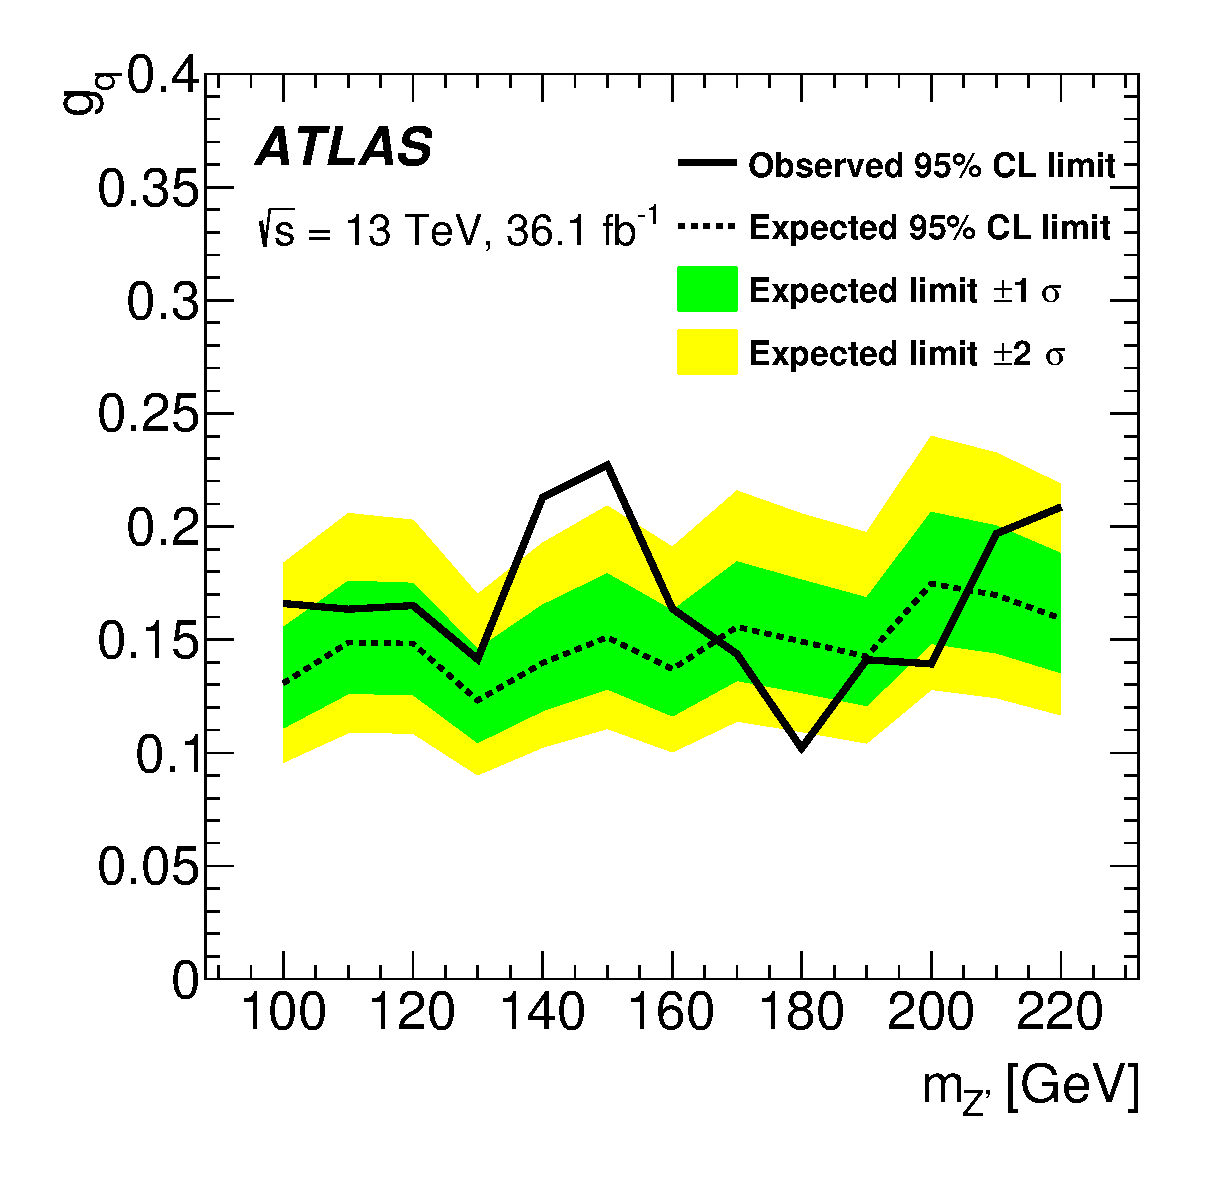
\includegraphics[width=\linewidth]{conclusions/untagged_analysis_g_q_limits.eps}
 \caption[Observed and expected limits at the $95\%$ confidence level on the coupling $g_{q}$ from the leptophobic axial-vector $\Zprime$ model for the combination of the ISR jet and ISR $\gamma$ channels of $\Zprime \to q\bar{q}+\mathrm{ISR}$.]{%
  Observed and expected limits at the $95\%$ confidence level on the coupling $g_{q}$ from the leptophobic axial-vector $\Zprime$ model for the combination of the ISR jet and ISR $\gamma$ channels of $\Zprime \to q\bar{q}+\mathrm{ISR}$~\cite{EXOT-2017-01}.
 }
 \label{fig:untagged_analysis_g_q_limits}
\end{figure}

\begin{figure}[htbp]
 \centering
 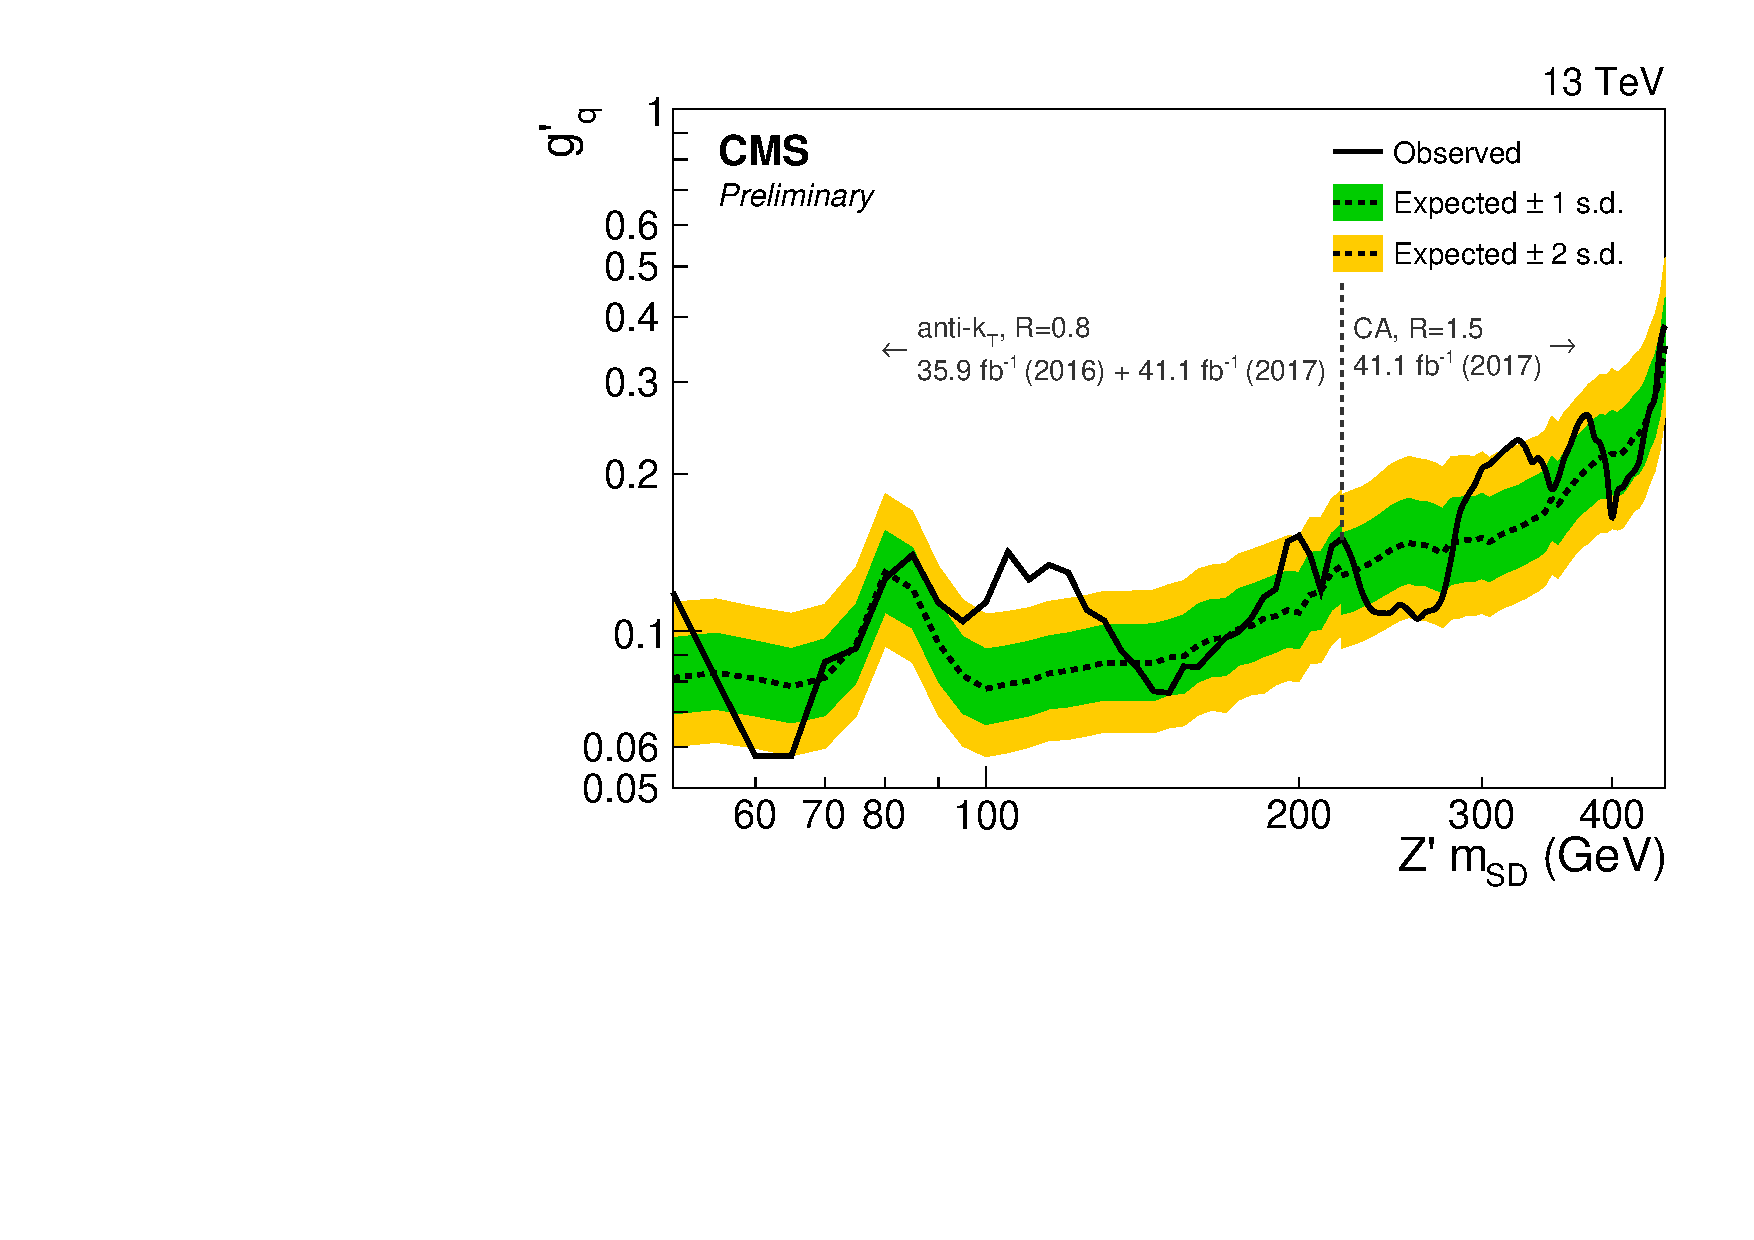
\includegraphics[width=\linewidth]{conclusions/CMS-PAS-EXO-18-012_Zprime_limits.pdf}
 \caption[CMS upper limits at $95\%$ CL on the coupling $g_{q}^{\prime}$ as a function of resonance mass for a leptophobic $\Zprime$ resonance that only couples to quarks using $77.0~\ifb$.]{%
  CMS upper limits at the $95\%$ confidence level on the coupling $g_{q}^{\prime}$ as a function of resonance mass for a leptophobic $\Zprime$ resonance that only couples to quarks.
  For masses between $50~\GeV$ and $220~\GeV$ the limits correspond to a $\Zprime$ resonance reconstructed in AK8 jets using $77.0~\ifb$ of statistically combined data from 2016 and 2017.
  The excess in the observed limit over the expected limit near $120~\GeV$ is a remnant of the analysis of the data collected in 2016.
  For masses above $220~\GeV$ up to $450~\GeV$ the results correspond to a $\Zprime$ resonance reconstructed in CA15 jets using $41.1~\ifb$ of data collected in 2017~\cite{CMS:2019hlx}.
 }
 \label{fig:CMS-PAS-EXO-18-012_Zprime_limits}
\end{figure}

This thesis analysis has been a successful step forward in bringing burgeoning techniques and new ideas to bear in exploring the wealth of data ATLAS collected in Run 2.
Equipped with this analysis as a tool for inference of Nature, it is with great excitement that I join the particle physics community in preparing for boosted searches of new physics in the upcoming Run 3 of the LHC.
